% LaTeX .tex example for the proceedings of
% COBEM 2015 - 23rd International Congress of Mechanical Engineering
% November, 6-11 2015 - Rio de Janeiro, RJ, Brazil
%
% Based on the template of the proceedings of COBEM2013 
%
% Max. 8 pg

\documentclass[10pt,fleqn,a4paper,twoside]{article}
\usepackage{cobem2015}

\usepackage{amsmath}
\usepackage{todo}
\graphicspath{ {./Figs/} }

\def\shortauthor{R. Corsi, J. Jaime}
\def\shorttitle{Active Magnetic Bearing Project For a Satellite Reaction Wheel}

\newcommand{\executeiffilenewer}[3]{%
	\ifnum\pdfstrcmp{\pdffilemoddate{#1}}%
	{\pdffilemoddate{#2}}>0%
	{\immediate\write18{#3}}\fi%
}

\newcommand{\includesvg}[1]{%
	\executeiffilenewer{#1.svg}{#1.pdf}%
	{inkscape -z -D --file=./Figs/#1.svg %
		--export-pdf=./Figs/#1.pdf --export-latex}%
	\input{./Figs/#1.pdf_tex}%
}


\begin{document}
	\fphead
	\hspace*{-2.5mm}\begin{tabular}{||p{\textwidth}}
		\begin{center}
			\vspace{-4mm}
			\title{ACTIVE MAGNETIC BEARING PROJECT FOR A SATELLITE REACTION WHEEL}
		\end{center}
		\authors{Rafael~Corsi~Ferr\~{a}o} \\
		\authors{Jos\'{e} Jaime da Cruz} \\
		\institution{Escola Polit\'ecnica da Cidade de S\~{a}o Paulo} \\
		\institution{corsiferrao@gmail.com, jaime@lac.usp.br} \\
		\\
		%\authors{Third Author's Name} \\
		%\institution{Institution and address for third author} \\
		%\institution{e-mail} \\
		%\\
		%\authors{Same format for others authors, if any} \\
		\\
		\abstract{\textbf{Abstract.} In this paper, the development of a novel active magnetic bearing (MB) system for reaction wheels applicable in satellite attitude control is presented. The proposed bearing has four degrees of freedom passively stable (EMB) by one pair of permanent magnet; two degrees of freedom (AMB) are actively stabilized by eight electromagnetic poles. The  magnetic model of both EMB and AMB are presented and  equations of force-current and force-position are analyzed by the magnetic circuit approach and by the finite element method. With the force characteristic curves a non-linear dynamic model for the MB and a control system that stabilizes the bearing at its operating point are presented. A flat, uncoupled and scalable magnetic bearing with good stiffness, that can be used on satellites reaction wheels to improve its performance and reliability, is obtained. A prototype is under construction. Simulation results are presented.}\\
		\\
		\keywords{\textbf{Keywords:} Magnetic Bearing, Satellite Attitude Control }\\
	\end{tabular}
	
	\section{INTRODUCTION}
	The attitude and orbit control is one of the most critical technology of any spatial systems \citep{wertz1978spacecraft}, the main actuators include propellants, magnetic torques and reaction wheels.  Reaction wheels are hard to replace because they present a large operating range in torque (unlike magnetic actuators) and are powered by renewable energy provided by solar panels (unlike propellers based on a finite fuel supply). For these reasons, reaction wheels are present on virtually any satellite that with a  minimum performance requirements in attitude.
	
	A reaction wheel can be described as an inertial actuator operating on the principle of conservation of angular momentum. The performance of the reaction wheel on the satellite takes place by exchange of angular momentum, limited to the axis of rotation of the wheel. Due to the large difference between the satellite and the inertia of the reaction wheel, a control of attitude with great precision is possible with this system.
	
	Reaction wheels typically consist of an electric motor, usually a DC brushless motor, a bearing system and one element of inertia. The inertia member and the motor are mounted on bearings to ensure precise rotation about an axis. The rotation speed of the system is controlled by an electronic motor drive. Reaction wheels can be operated in two distinct ways: by rotation or torque. When torque commanded by the reaction wheel should be able to estimate the useful torque generated by it (the effective torque less losses).
	
	The suspension of the rotor relative to the stator is a critical part in the reaction wheels \cite{taniwaki2003experimental} because the consequences of any friction in the relative movement between these two components. Indeed, the friction is reflected not only in a greater consumption of electric power, as well as the introduction of a dead zone of operation in torque as well as the limited life of the reaction wheel due to gradual wear of the bearing.
	
	A  mechanical solution for the interface between the rotor and the stator is a rolling bearing. Despite its apparent simplicity, presents challenges for achieving the minimum friction values needed in view of the demands of consumption, controllability and life of the reaction wheel \cite{Krishnan2010}. In the case of aerospace applications, lubrication rolling is also considerable difficulty due to the impossibility of using traditional lubricants under conditions of low or no air pressure, which leads to loss of volatile components such lubricants and their consequent deterioration. Another difficulty is due to the trend of migration of lubricants in the absence of gravity, which is usually addressed with strategies to recapture or lubrication. Lubrication systems in particular, have great complexity and its orbital behaviour is difficult in the laboratory validation.
	
	Another solution is to use a magnetic bearing \cite{Bangcheng2012}, which is an alternative without mechanical contact between the rotor and the stator, wherein the rotor is suspended magnetically maintained. The gain in reliability and lifetime of the reaction wheel is considerable \cite{Marble2006}, and life basically limited by the durability of electronics. The non-contact operation eliminates the need for lubrication and consequently enables the operation under vacuum which results in simplifying the mechanical design requirements.
	
	\subsection{Magnetic Bearing for Reaction Wheel}
	
	There is in the literature three different topologies for use in bearings in magnetic reaction wheels, bearings proposed for this type of application have mostly two degrees of freedom active, and makes use of magnets standing for generating magnetic fields to minimize power consumption active electrical system. 
	
	The topology proposed by \cite{Bernus 1998} works with two degrees of assets liberties having the permanent magnets on the rotor and two stators, on this proposition, the radial direction is unstable and must be active controlled. The rotor has a "I" cross shape and it is surrounded by the external stator with an "C" cross shape, the internal ring is also an "C" shape. The internal stator is used for active control the radial directions of the rotor, it has four independent poles to generate magnetic flux, this flux also contributes to increase the axial stiffness of the rotor. The magnetic flux that is generated by magnetics on the rotor has it path through the external and internal stator generating a restorative force in case of an axial displacement.
	
	Another magnetic bearing proposition is from \cite{Scharfe2001} also works with the radial direction active controlled, it has only one stator that is located at the center of the bearing and one external rotor, both parts have a "C" cross shape. The permanent magnetic poles are located on the rotor generating a magnetic flux that stabilizes the axial direction, the internal stator can generate an attractive force to stabilizes the radial direction but the same magnetic flux that stabilizes the axial direction also generates an attractive force on the radial direction, this force must be overcome by the internal stator in order to place the rotor on its operation point, this topology allows generating a subtractive magnetic flux in some parts of the rotor in favor of decrease the attraction force and places the rotor at the operation point with less effort. 
	
	A recent topology is proposed by \cite{Bangcheng2012} with  three degree of freedom projected for a agile satellite, the focus of this topology is to supplies an substantial axial stiffness (passive axis) in order to maintain the rotor on its operation point when applied to  gyroscope effect.
		
	\section{Project}
	
	The magnetic bearing proposed in this work is in parts a junction topologies by \cite{Bernus1998} and \cite{Scharfe2001}. The bearing has four degrees of freedom passively stable: tilt, row, pitch and its axial direction, the other two degrees of freedom (the radial displacement) are actively stabilized. The torque imposed for the rotation of the rotor is not addressed in this paper but will be developed by an electric motor brushless DC (BLDC) placed inside the bearing. The magnetic circuit comprises two stators: one inner rotor and an outer rotor. The outer stator is responsible for the stabilization of the passives degrees of freedom and the inner one to active control the radial position through eight magnetic poles. Was decided to install the permanent magnets in the external stator not in the rotor as seen in the literature, seeking to the best mechanical balance of the rotor.
	
	Figure \ref{fig:mancal:corte} illustrates the proposed bearing. We adopted a flat geometry to better stiffness in the unstable modes of the bearing. The outboard bearing to the motor enables a rigidity within the proposed limits of mass and dimensions.
	
	\begin{figure}[ht]
		\centering
		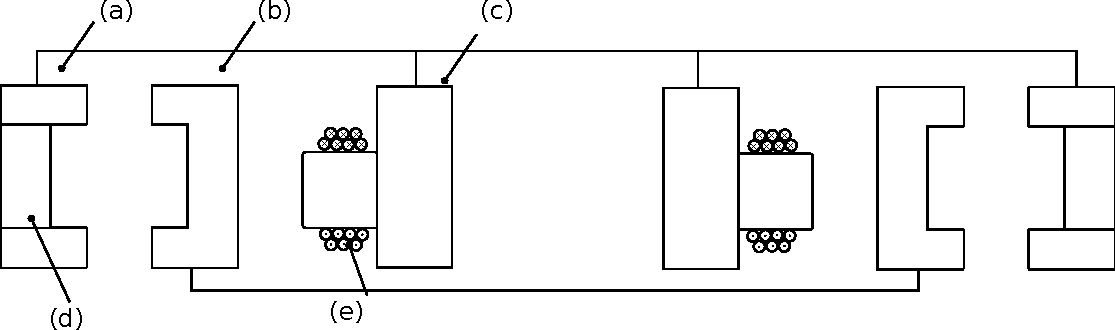
\includegraphics[width=1\linewidth]{Figs/mancais/mancal_corte2}
		\caption{Radial cut of the proposed magnetic bearing. (a) External stator; (b) Rotor; (c) Internal stator; (d) Permanent magnetics; (e) Coils}
		\label{fig:mancal:corte}
	\end{figure}
	
	\subsection{External Stator and Rotor}
	
	The magnetic circuit of a section of the outer stator is illustrated in Figure \ref{fig:circuito:passivo}. We found that the magnetic flux generated by the permanent magnet seeks the path of the least reluctance to close the magnetic circuit. This occurs by way of the external stator irons, then passing through the air gap and rotor. The permanent magnetic is a magnetic field source ($ F_ {ima} $) and is located between two irons. 
	The rotor undergoes attraction on all direction, at equilibrium (with a symmetrical air gap) the force resultant would tend to be null and the rotor remain in equilibrium at the operating point (critically stable). 
	
	\begin{figure}[ht]
		\centering
		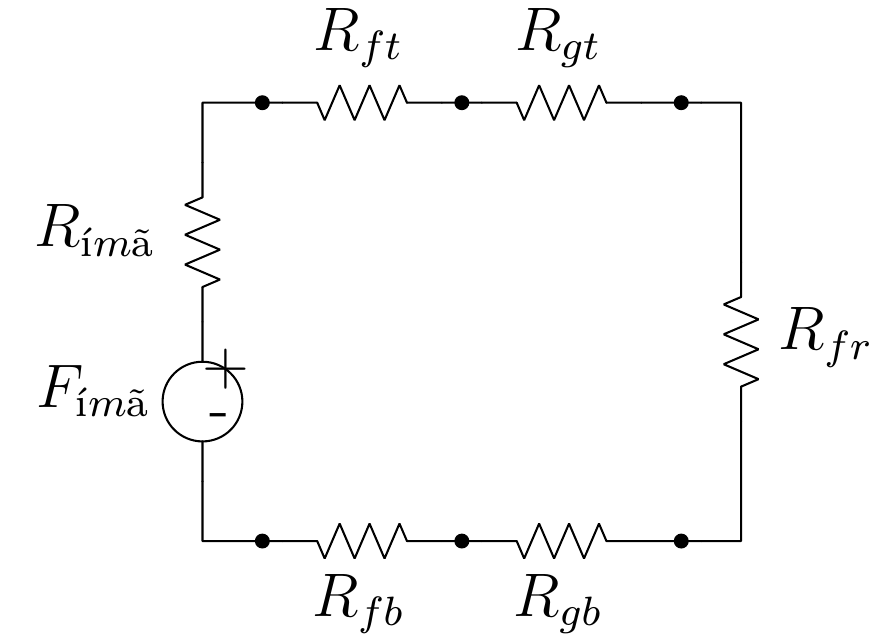
\includegraphics[width=0.4\linewidth]{Figs/circuito_passivo}
		\caption{Magnetic circuit of the outer stator and rotor}
		\label{fig:circuito:passivo}
	\end{figure}
	
	Aiming the linearisation of the attractive force on the radial displacement, the  outer stator irons are project to work always saturated, with this the magnetic field becomes almost constant for small changes in the air gap so that the no-linear component on the magnetic attractive force ($F = \frac{B^2 \, S}{2 \mu_0}$) becomes substantially constant, making the force proportional do the air gap area (S). Besides the linearisation, it was possible to obtain a higher axial stiffness without a large increase in radial stiffness, which would require greater energy to stabilize the active part.
	
	The cumulative magnetic field in the air gap (generated by the permanent magnetic) can be decomposed into components $B_x$ and $B_z$ that are dependent on the displacement of the rotor $\Delta_x$ and $\Delta_z$, this shift implies also an increase in the length of the gap. The attraction force of the rotor by the stator is generated by the accumulated electromagnetic energy in the air gap, this force can then be calculated using the virtual work \citep{Chiba}. Fig. \ref{Fig:modelo:passivo:DxDz} illustrate the magnetic flow on the external stator when displaced radially. 
	
	\begin{figure}[ht]
		\centering
		\def\svgwidth{0.4\columnwidth}
		\includesvg{modelo_passivo_DxDy}
		\caption{Deslocamento em X e Y}
		\label{Fig:modelo:passivo:DxDz}
	\end{figure}
	
	In order to stabilizes the tilt, the bearing must have a $F_z$ superior  than $F_x $ for some angle range otherwise the tilt would cause a non symmetric force on the rotor making it unstable on tilt. 
	
	With an analytical model it was possible to choose the initial dimensions of the bearing, a finite element model was created and simulations performed in order to get a good  axial rigidity and a small component radial force. A map of the radial force magnitude in the x, y is illustrated in Fig. 3.9,  note that around the operating point the resultant force is practically null. But when the rotor is in some of its ends, the force of attraction is of the order of hundreds of Newton which will influence the definition of the active circuit that has to be able to overcome this force.
	
	\begin{figure}[th]
		\centering
		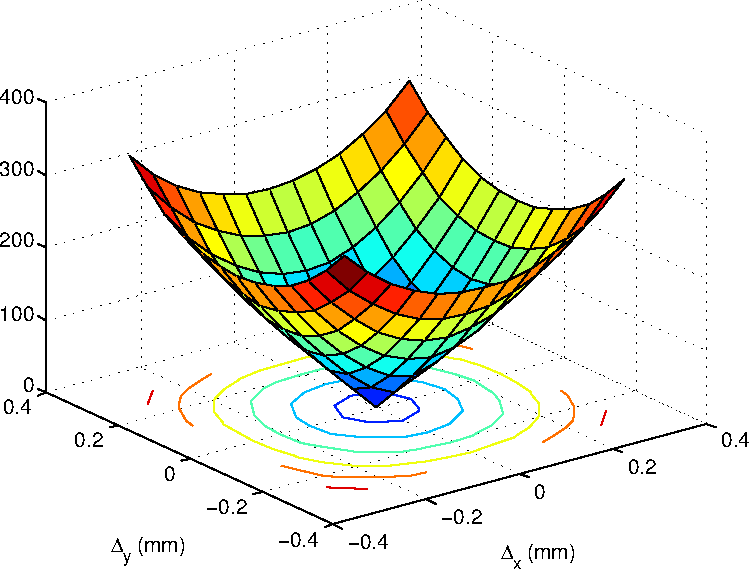
\includegraphics[width=0.5\linewidth]{./Figs/Simulacoes/Passivo/forca_passivo_mod_fx_fy_3d}
		\caption{3D map of attraction force on the radial direction due to passive bearing system}
		\label{fig:forca:passivo:mod:fx:fy:3d}
	\end{figure}
	
	The Fig. \ref{fig:forca:passivo:comsol:dy} is the result of forces in the rotor when subjected to an axial displacement,  found that the force has a component different from zero when the rotor is aligned with the external stator (z = 0), this is caused by numeric errors on the FEM analysis. The achieved magnetic rigidity force for the axial displacement is of 20N/mm and for the radial displacement is of 60N/mm. 
	
	\begin{figure}[ht]
		\centering
		{\textit{Magnetic Force (N) x Displacement Y (mm): Equilibrium point}}\\
		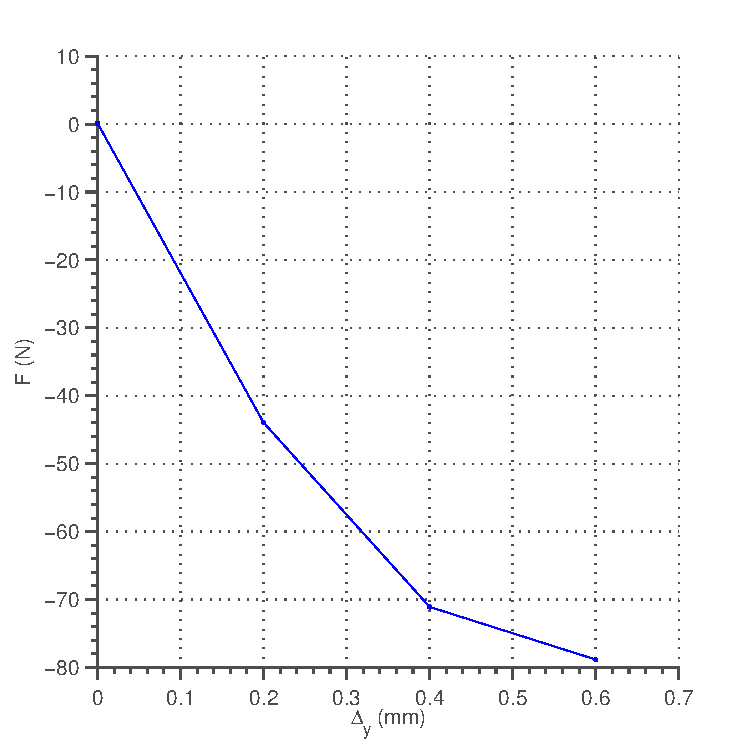
\includegraphics[width=0.4\linewidth]{./Figs/Simulacoes/Passivo/forca_passivo_comsol_dy}
		\caption{Passive stiffness for a axial displacement }
		\label{fig:forca:passivo:comsol:dy}
	\end{figure}
	
	\subsection{Inner stator and Rotor}
	
	The inner stator is formed with eight poles evenly distributed every 45 degrees, and connected by a ring of internal circulation. The poles function as actuators (electromagnets) to stabilize the rotor on the radial direction (x, z).  It is designed to always act with three poles assets, this approach makes the flow of the magnetic field that travels through the rotor is maximized in the shaft where it is desired to realize the attraction.
	
	Figure \ref{fig:modelo:mancal:estator:interno:fluxo} shows the internal stator with three poles of its assets: (A), (B), (C) and the flow flowing through the rotor generated by a current applied on the coils. The poles (A) and (C) in this example work with inverse polarity of (B) forcing the flow passing by (B) and not by any other pole, thus maximizing the force of attraction $F_B$. A part of the magnetic field flux does not pass by (B) and closes by other poles but can be despised due to its low component. The induced current flow in (A) and (C) is half the current in the main pole (B) this is done to prevent the pole (B) reaches saturation, since the field that crosses it comprises its owns flux plus the flux generated by the coils adjacent. 
	
	The generated forces $F_A$ and $F_C$  have components in both directions x and y, but for small displacement from the equilibrium point, the components in the y direction can be canceled as they are of the same intensity but in the opposite direction. Leading to a single force in the X direction compost by: $F_x = F_B + F_{Ax} + F_{Cx}$
	
	\begin{figure}[ht]
		\centering
		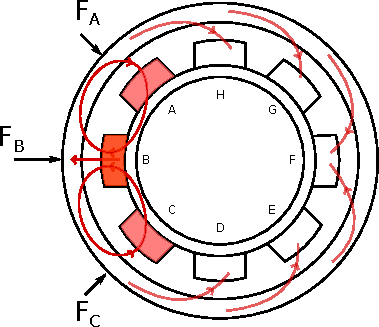
\includegraphics[width=0.5\linewidth]{./Figs/modelo_mancal_estator_interno_fluxo}
		\caption{Magnetic flux of active bearing system where A to H are the inner stator poles}
		\label{fig:modelo:mancal:estator:interno:fluxo}
	\end{figure}
	
	The magnetic circuit between the inner stator and the rotor can be seen in Figure \ref{fig:modelo:circuito:ativo:explicativo}, the circuit can be split on four main elements: The coil magnetic field generating source (c) the reluctance of the air gap which depends on the distance between the rotor poles and (b), the reluctance of the iron of the rotor (a) and the iron of the return ring (d).
	
	\begin{figure}[ht]
		\centering
		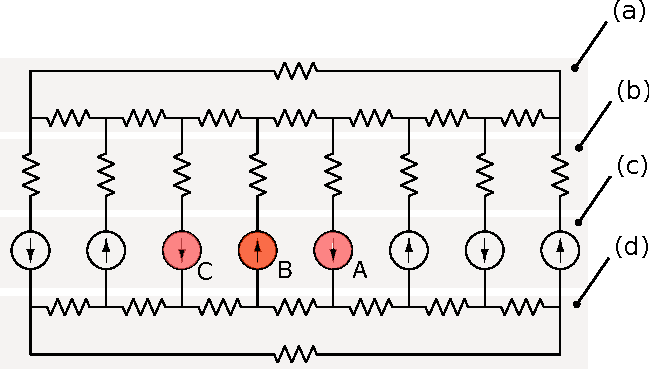
\includegraphics[width=0.5\linewidth]{./Figs/modelo_circuito_ativo_explicativo}
		\caption{Electromagnetic circuit of inner stator and rotor. (a) rotor reluctance, (b) airgap reluctance, (c) magnetic flux generate by the poles, (d) return ring}
		\label{fig:modelo:circuito:ativo:explicativo}
	\end{figure}
	
	
	The forces can be calculated by the principle of virtual work, this forces are decomposed in the two main axes (x, y). For small rotor displacement is possible to approximate this decomposition and get the attraction force: 
	
	\begin{align}
		\vec{F}_x &= \vec{F}_{gn} + \cos(45) (\vec{F}_{ga} + \vec{F}_{gb}) \label{eq:ativo:F:resultante:y} \\
		\vec{F}_y &=  \cos(45) (\vec{F}_{ga} - \vec{F}_{gb}) = 0 \label{eq:ativo:F:resultante:x}
	\end{align}
	
	The geometric parameters of the internal stator were raised starting from the restriction imposed by the power specifications. The maximum power for the system is 100W with a  supply voltage of 24V, obtain the maximum possible current  (4A). This electric current must be sufficient to generate a attraction force to compensate the force generated by the passive circuit (permanent magnetics) in the largest  possible gap, raised in the finite element model (160N).
	
	From the magnetic force equation \eqref{eq:ativo:F:resultante:y} is possible to draw an approximation of the area needed to reach the necessary force to move the rotor from the worst case possible (with the maximum air gap). The magnetic flux density used on this model is the maximum possible flux (saturation) of the 1020 steel (1.5T). With an initial value of the lateral pole area, was defined the number of turns of coils required to generate the magnetic flux in the air gap. From the number of coils it was possible to determine the pole length to support this coins. Figure \ref{fig:magnetico:ativo:comsol} shows the achieved attraction force due the inner stator poles.
	
	\begin{figure}
		\centering
		Force (N) x Current (A) at maximum air gap\\
		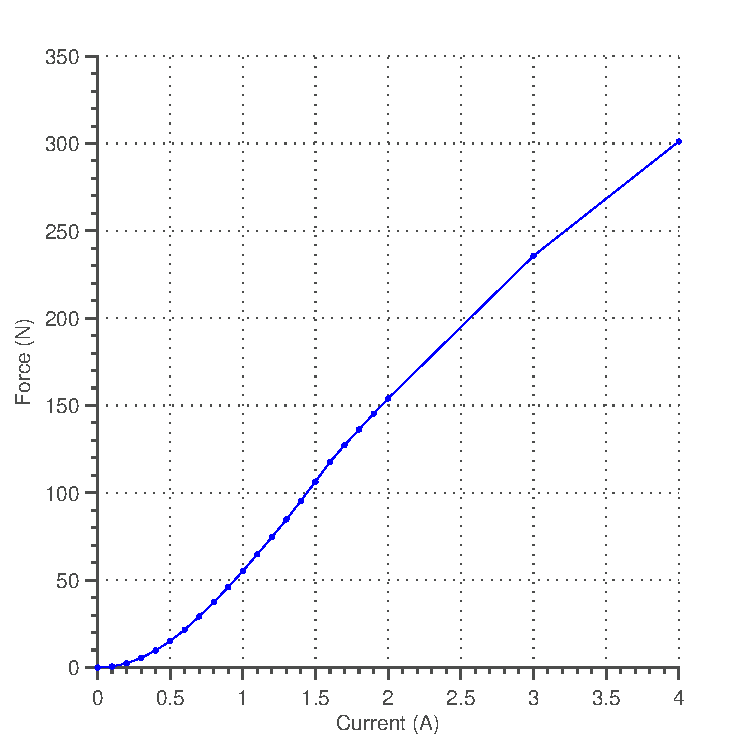
\includegraphics[width=0.4\linewidth]{/Simulacoes/Ativo/Forca_ativo_artigo}
		\caption{Attraction force at maximum air gap }
		\label{fig:magnetico:ativo:comsol}
	\end{figure}
	
	\subsection{Indutance} \label{subsec:at:indutancia}
	
	The calculation of inductance is important because it impose a dynamic to the actuator also it can be used to as a mean to measurement the rotor displacement position. Inductance is correlated with generation capacity of magnetic flux in a coil and its current, It is defined by:
	
	\begin{equation}
		L = \frac{d \phi}{di} .
	\end{equation}
	
	The achieved inductance for each coils is of $56 mH$ with a electrical resistance of $4 \Omega$. Increasing the size of the coil generates a positive gain on the attraction force but decreases the cut-off frequency, implying a slower actuators and complex control system.
	
	\subsection{Auxiliary Bearing}
	
	Auxiliary bearings are essential on any magnetic bearing, it prevents the shock between the rotor and any critical part when the magnetic bearing is disabled or on a failure situation. The proposed auxiliary bearing is a solid bearing that prevents the shock between irons (rotor and inner or outer stator), it also limited the rotor tilt angle not allowing it to get on a non stable zone (where the radial attraction force is greater than the axial force).
	1	
	\subsection{Bearing dimensions}
	
	The achieved magnetic bearing has an external radio of 75.8 mm and height of 18.0 mm. The nominal air gap between the rotor and the external stator is of 1.2mm and of 0.6 between rotor and inner stator. 
	
	\section{Dynamic Model}
	
	Via Lagrangian formalism we obtain the portion of the kinetic energy (T) from the rotor that results from the rotation of the rotor and it displacement. The potential energy (V) is due to axial translation of the rotor (in an environment with gravity): 
	
	\begin{align}
		T_{\theta, x, y, z} &= \frac{1}{2} I_z \, \dot{\theta}^2 + \frac{1}{2} \, m \, \left( \dot{x}^2 + \dot{y}^2 + \dot{z}^2 \right) \notag \\
		V_z &= m \, g \, z + \frac{1}{2} \, K \, z^2
	\end{align}
	
	There are two types of forces acting on the rotor, the  non-conservative forces ($Q^{nc}$) that are caused by the active part of the bearing and the conservative ($Q^{c}$) forces (which depend only on the position of the rotor) are result of the passive bearing part.
	
	\begin{align}
		Q_y^{nc} &= F_{by}(x,y,i)  \\
		Q_x^{nc} &= F_{bx}(x,y,i)  \\
		Q^{c}_x &= K_p \, x \\
		Q^{c}_y &= K_p \, y 
	\end{align}
	
	Is possible to obtain the differential equations that govern the model:
		
	\begin{align}
		I \ddot{\theta} &= 0 \\
		m \ddot{x}		&=  F_{px}(x,y) - F_{by}(x,y,i) \\
		m \ddot{y}		&=  F_{py}(x,y) - F_{bx}(x,y,i)\\	
		m \ddot{z} - K z &= m g  + F_{pz}
	\end{align}
	
	%\subsection{Actuator Dynamic}
	
	The actuator dynamics is generated primarily by the coils,  this inductance is time-varying since it depends on the rotor position. On this linear model we used the worst case model (largest inductance) which has a cut-off frequency of $11Hz$. The actuator dynamic is than :
	
	\begin{align}
		\frac{I(s)}{V(s)} = G_a(s) = \frac{1}{R + L \, s} = \frac{V(s)}{4 + 0.056 \, s}
	\end{align}
	
	The block diagram for the radial rotor displacement is shown on Fig. \ref{fig:diagrama:blocos:modelo:linear}.
	
	\begin{figure}[th!]
		\centering
		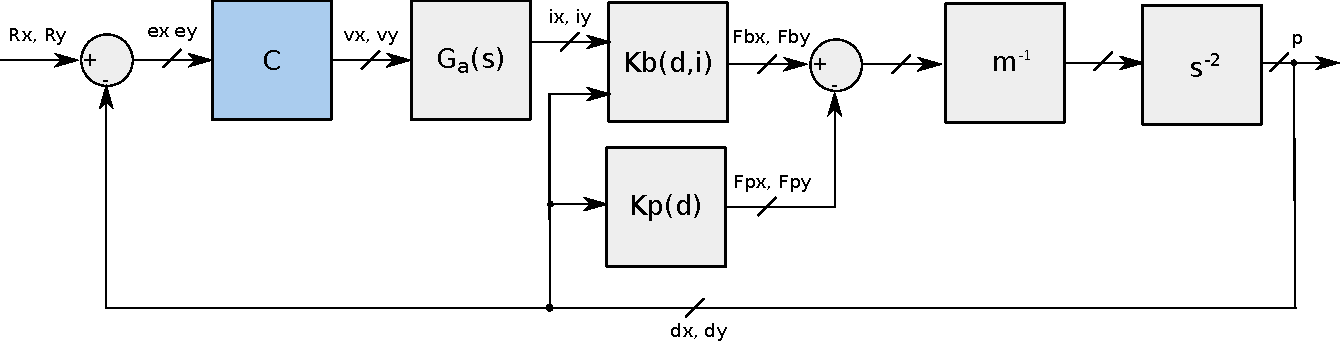
\includegraphics[width=1\linewidth]{../Figs/Modelagem/diagrama_blocos_modelo_linear}
		\caption{Diagrama de blocos do modelo linearizado para descolamentos em x e y}
		\label{fig:diagrama:blocos:modelo:linear}
	\end{figure}
	
	\section{Control}
	
	\section{ACKNOWLEDGEMENTS}
	
	This optional section must be placed before the list of references.
	
	\section{REFERENCES} 
	
	\bibliographystyle{cobem2015}
	\renewcommand{\refname}{}
	\bibliography{./bibfile}
	
	\section{RESPONSIBILITY NOTICE}
	
	The authors are the only responsible for the printed material included in this paper.
	
\end{document}
